%\documentclass{beamer}
\documentclass[handout]{beamer}
% This file is a solution template for:

% - Giving a talk on some subject.
% - The talk is between 15min and 45min long.
% - Style is ornate.

% Copyright 2004 by Till Tantau <tantau@users.sourceforge.net>.
%
% In principle, this file can be redistributed and/or modified under
% the terms of the GNU Public License, version 2.
%
% However, this file is supposed to be a template to be modified
% for your own needs. For this reason, if you use this file as a
% template and not specifically distribute it as part of a another
% package/program, I grant the extra permission to freely copy and
% modify this file as you see fit and even to delete this copyright
% notice. 

\mode<presentation>
{
  \usetheme{Montpellier}

  %\setbeamercovered{transparent}
  % or whatever (possibly just delete it)
}

\usepackage{xmpmulti} % package that defines \multiinclude

\usepackage[english]{babel}

\usepackage[latin1]{inputenc}

\usepackage{times}
\usepackage[T1]{fontenc}
% Or whatever. Note that the encoding and the font should match. If T1
% does not look nice, try deleting the line with the fontenc.

\title [Multi-arm Bandits] %(optional, use only with long paper titles)
{Online learning using limited feedback}

\author[Freund] % (optional, use only with lots of authors)
{Yoav Freund}
% - Give the names in the same order as the appear in the paper.
% - Use the \inst{?} command only if the authors have different
%   affiliation.

\institute[Universities of Somewhere and Elsewhere] % (optional, but mostly needed)

\subject{Machine Learning}
% This is only inserted into the PDF information catalog. Can be left
% out. 

% If you have a file called "university-logo-filename.xxx", where xxx
% is a graphic format that can be processed by latex or pdflatex,
% resp., then you can add a logo as follows:

% \pgfdeclareimage[height=0.5cm]{university-logo}{university-logo-filename}
% \logo{\pgfuseimage{university-logo}}



% Delete this, if you do not want the table of contents to pop up at
% the beginning of each subsection:
%% \AtBeginSubsection[]
%% {
%%   \begin{frame}<beamer>
%%     \frametitle{Outline}
%%     \tableofcontents[currentsection,currentsubsection]
%%   \end{frame}
%% }


% If you wish to uncover everything in a step-wise fashion, uncomment
% the following command: 

\beamerdefaultoverlayspecification{<+->}

\newcommand{\newmcommand}[2]{\newcommand{#1}{{\ifmmode {#2}\else\mbox{${#2}$}\fi}}}
\newcommand{\newmcommandi}[2]{\newcommand{#1}[1]{{\ifmmode {#2}\else\mbox{${#2}$}\fi}}}
\newcommand{\newmcommandii}[2]{\newcommand{#1}[2]{{\ifmmode {#2}\else\mbox{${#2}$}\fi}}}
\newcommand{\newmcommandiii}[2]{\newcommand{#1}[3]{{\ifmmode {#2}\else\mbox{${#2}$}\fi}}}

\newcommand{\algfnt}{\bf}

\newmcommand{\ouralg}{{\mbox{\algfnt Hedge}({\eta})}}

\newmcommand{\iter}{T}

\newfont{\cmmib}{cmmib10}
\newcommand{\boldell}{{\mbox{\cmmib \symbol{'140}}}}

\newmcommandi{\costvec}{{\boldell}^{#1}}
\newmcommandii{\cost}{{\ell}^{#1}_{#2}}

\newmcommandi{\rd}{\tilde{#1}}

\newmcommandi{\distvec}{{\bf p}^{#1}}
\newmcommandi{\rddistvec}{\rd{\bf p}^{#1}}
\newmcommandii{\dist}{{p}^{#1}_{#2}}
\newmcommandii{\rddist}{\rd{p}^{#1}_{#2}}

\newmcommandi{\bdistvec}{{\bf q}^{#1}}
\newmcommandii{\bdist}{{q}^{#1}_{#2}}

\newmcommandi{\wtvec}{{\bf w}^{#1}}
\newmcommandi{\rdwtvec}{\rd{\bf w}^{#1}}
\newmcommandii{\wt}{{w}^{#1}_{#2}}
\newmcommandii{\rdwt}{\rd{w}^{#1}_{#2}}

\newcommand{\w}[1]{\makebox[12pt]{{#1}}}
\newcommand{\Rps}{\mbox{\tt R}}
\newcommand{\rPs}{\mbox{\tt P}}
\newcommand{\rpS}{\mbox{\tt S}}
\newcommand{\rpstie}{\w{$\frac{1}{2}$}}
\newcommand{\rpswin}{\w{$0$}}
\newcommand{\rpsloss}{\w{$1$}}

\newmcommand{\decspace}{\Delta}
\newmcommand{\decsym}{\delta}
\newmcommandi{\dec}{\decsym^{#1}}
\newmcommand{\decdistsym}{\cal D}
\newmcommandi{\decdist}{{\decdistsym}^{#1}}

\newmcommand{\simpdistspace}{{\bf \cal S}}
\newmcommand{\domset}{{\rm dom}(\decdistsym)}

\newmcommand{\expdistsym}{{\cal E}}
\newmcommandii{\expdist}{{\expdistsym}^{#1}_{#2}}
\newmcommand{\expdecsym}{{\varepsilon}}
\newmcommandii{\expdec}{\expdecsym^{#1}_{#2}}

\newmcommand{\outspace}{\Omega}
\newmcommand{\outsym}{\omega}
\newmcommandi{\out}{\outsym^{#1}}

%\newmcommandii{\Dkl}{D_{\mbox{kl}}\paren{#1||#2}}
\newmcommandii{\Dkl}{{\rm {KL}}\paren{{#1}\;||\;{#2}}}

\newmcommandi{\sumwts}{\sum_{i=1}^N \wt{#1}{i}}

\newmcommand{\lossalg}{L_A}
\newmcommand{\lossouralg}{{L_{\mbox{\scriptsize\algfnt Hedge}(\eta)}}}
\newmcommand{\lossS}{{L_{\mbox{\scriptsize\algfnt S}}}}
\newmcommandi{\lossi}{L_{#1}}
\newmcommandii{\lossit}{L_{#1}^{#2}}

\newmcommandi{\upbnd}{\tilde{#1}}

\newcommand{\angles}[1]{{\left\langle {#1} \right\rangle}}
\newcommand{\paren}[1]{{\left( {#1} \right)}}
\newcommand{\abs}[1]{{\left| {#1} \right|}}
\newcommand{\ceiling}[1]{{\left\lceil {#1} \right\rceil}}

\newfont{\msym}{msbm10}
\newcommand{\real}{\mbox{\msym R}}

\newmcommand{\updatefcn}{U_\eta}

%% \newtheorem{theorem}{Theorem}	
%% \newtheorem{lemma}[theorem]{Lemma}
%% \newtheorem{corollary}[theorem]{Corollary}
%% \newtheorem{definition}{Definition}

%\newcommand{\proof}{\noindent{\bf Proof:} }
%\newcommand{\example}[1]{{\em Example #1.} }
%\newcommand{\qed}{\rule{0.7em}{0.7em}}

\newcommand{\WeakAlg}{\mbox{\algfnt WeakLearn}}
\newcommand{\Boost}{\mbox{\algfnt AdaBoost}}
\newcommand{\EX}{\mbox{\bf EX}}
\newmcommand{\hf}{h_{{f}}}
\newmcommand{\rdhf}{\rd{h}_{{f}}}
\newmcommand{\hfT}{h^T_{{f}}}
\newmcommand{\ranh}{{b}}

\newmcommand{\conclass}{{\cal C}}

\newmcommand{\badvec}{{\bf b}}
\newmcommandi{\bad}{{b}_{#1}}

%%%%%%%% New commands defined for the game-playing paper

\newmcommand{\hedge}{\algfnt Hedge}
\newmcommand{\play}{\algfnt Play}
\newmcommandi{\Glossvec}{{\bg y}^{#1}}
\newmcommandii{\Gloss}{{y}^{#1}_{#2}}
%\newmcommandi{\action}{{I}_{#1}}
\newmcommandi{\Gdistvec}{{\bf \tilde{p}}^{#1}}
\newmcommandii{\Gdist}{{\teilde{p}}^{#1}_{#2}}

%%%%%%%%%%%%%%%%%%%%%%%%%%%%%%%%%%%%%%%%%%%%%%%%%%%%%
\newmcommand{\Idistvec}{{D}}
\newmcommandi{\Idist}{\Idistvec({#1})}
\newmcommand{\Idistt}{\Idistvec_t}

\newmcommand{\Xdist}{{\cal P}}
\newmcommand{\emp}{\hat{\epsilon}}

\newmcommand{\classpc}{Y}
\newmcommand{\numclass}{k}
\newmcommandii{\prob}{\mbox{\rm Pr}_{#1}\left[{#2}\right]}
\newmcommandii{\exval}{\mbox{\rm E}_{#1}\left[{#2}\right]}

\newmcommand{\lab}{y}
\newmcommand{\ploss}{\mbox{ploss}}
\newmcommandii{\avploss}{\ploss_{#1}({#2})}
\newcommand{\sfrac}[2]{\mbox{$\frac{#1}{#2}$}}

\newcommand{\mboosta}{\mbox{\algfnt AdaBoost.M1}}
\newcommand{\mboostb}{\mbox{\algfnt AdaBoost.M2}}
\newcommand{\mboostr}{\mbox{\algfnt AdaBoost.R}}

\newmcommand{\slos}{\mbox{ploss}}
\newmcommandiii{\sloss}{\slos_{#1}({#2},{#3})}
\newmcommandiii{\avsloss}{\slos_{{#1},{#2}}({#3})}

\newmcommandii{\vwt}{{W}^{#1}_{#2}}

\newcommand{\figline}{\rule{\textwidth}{1pt}}

%\newmcommandi{\1}{{\bf 1}({#1})}
\newmcommandi{\1}{[\![{#1}]\!]}

\newmcommand{\confcn}{\kappa}
\newmcommandi{\erint}{\abs{\int_{y_i}^{h_t(x_i)} {#1} dy}}
%\newmcommandi{\erint}{\int_{\min\{y_i,h_t(x_i)\}}^{\max\{y_i,h_t(x_i)\}}{#1}dy}

\newcommand{\blue}[1]{{\color{blue}{#1}}}
\newcommand{\red}[1]{{\color{red}{#1}}}
\newcommand{\redEq}[1]{{\color{red}{$#1$}}}
\newcommand{\W}{\vec{W}}
\newcommand{\V}{\vec{V}}
\newcommand{\X}{\vec{X}}
\newcommand{\loss}{\vec{\ell}}
\newcommand{\HedgeLoss}{L_{\mbox{\footnotesize Hedge}}}


\begin{document}

\iffalse %%%%%%%%%%%%%%%%%%%%%%%%%%%%%%%%%%%%%%%%%%%%%%%%%%%%%%%%%%%%%%%%%%
\fi %%%%%%%%%%%%%%%%%%%%%%%%%%%%%%%%%%

\begin{frame}
  \titlepage
\end{frame}

\begin{frame}
  \frametitle{Outline}
  \tableofcontents[pausesections]
  % You might wish to add the option [pausesections]
\end{frame}

\section{The multiple-arm bandits problem}

\begin{frame}
\frametitle{The one armed bandit}
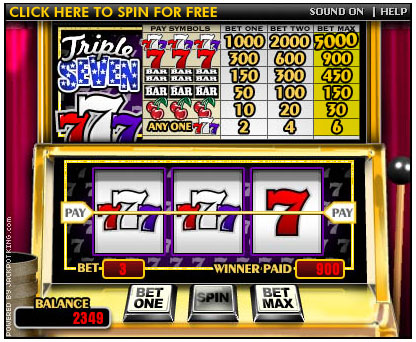
\includegraphics[width=8cm]{figures/OneArmBandit.jpg}
\end{frame}

\begin{frame}
\frametitle{The multiple arm bandit problem}
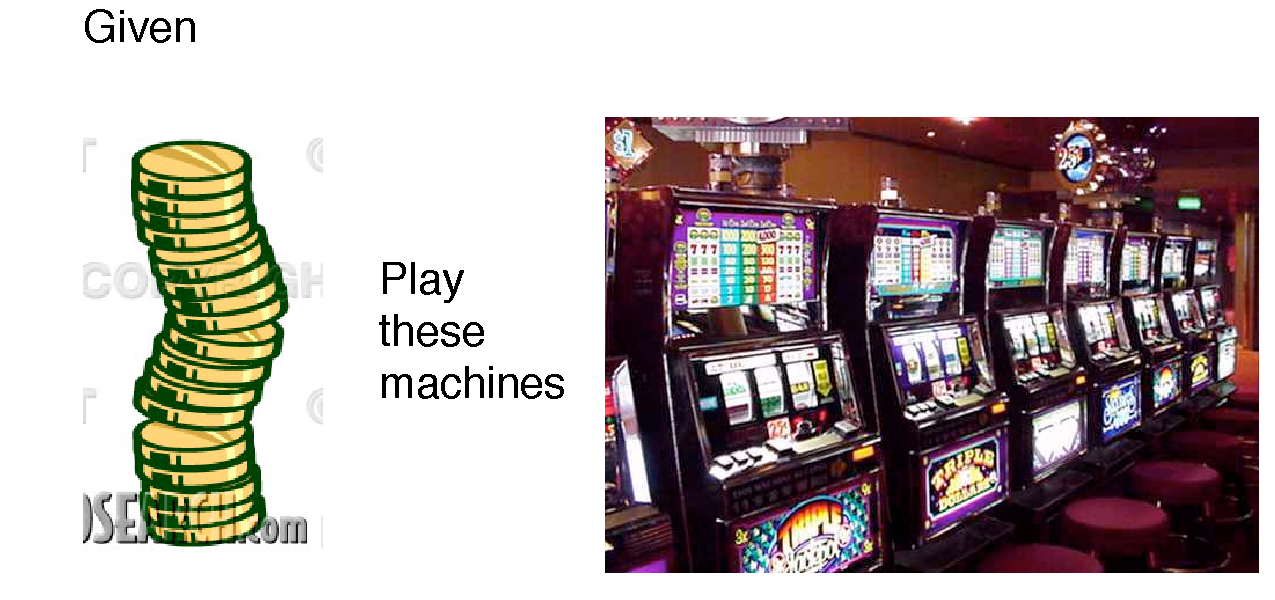
\includegraphics[width=8cm]{figures/multiArm.pdf}
\\
\pause
\B{Goal:} Maximize expected wealth.\\
\pause
Mathematical formulation for common \\
\B{Exploration vs. Exploitation} dilemma.\\
\pause
\B{single-iteration reward} is in the range \R{$[0,1]$}
\end{frame}


\section{The classical analysis - Gittins Index}

\begin{frame}
\frametitle{Classical analysis}
\begin{itemize}
\item Rewards generated \B{independently at random}
\item Each machine has a different distribution of rewards.
\item \B{Basic idea:} sample so as to minimize uncertrainty in identity of
  best arm.
\end{itemize}
\end{frame}

\section{The adversarial setup}

\begin{frame}
\frametitle{Playing in a Rigged casino}
\begin{itemize}
\item The casino operator watches you and changes rewards of the
  machines to \B{confuse} you!
\item Can you still find the best machine?
\item What does \B{``best machine''} mean?
\end{itemize}
\end{frame}

\begin{frame} 
\frametitle{Example adversarial MAB game} 

\begin{columns} 
\column[t]{2cm}
\onslide<1->\color<1>{red}
~\\  action1\\ action2\\ action3\\ action4 \\ action5\\ action6\\ action7\\ action8 
\column[t]{1cm}
\onslide<2->\color<2>{red} $P_1$ \\  $1/8$ \\  $1/8$  \\  $1/8$  \\  $1/8$  \\  $1/8$ \\  $1/8$ \\  $1/8$  \\  $1/8$ 
\column[t]{1cm}
\onslide<3->\color<3->{blue} $\i{1}$ \\  ~ \\  ~  \\  ~  \\  $\Rightarrow$  \\ ~  \\  ~  \\  ~  \\ ~   
\column[t]{1cm}
\onslide<4->\color<4>{red}{ $\xv{1}$ \\ .1 \\ .8  \\ .3  \\ \B{.5}  \\ .9 \\  0 \\  1  \\ .8 }

\column[t]{1cm}
\onslide<5->\color<5>{red}{ $p_2$ \\  .12\\  .12\\.12 \\ .16 \\ .12\\  .12 \\ .12 \\ .12 }
\column[t]{1cm}
\onslide<6->\color<6->{blue} $\i{2}$ \\  ~ \\  ~  \\  ~  \\  ~  \\ ~  \\  ~  \\  $\Rightarrow$  \\ ~   
\column[t]{1cm}
\onslide<7->\color<7>{red}{ $\xv{2}$ \\ .1 \\ .5 \\ .2  \\ .7 \\ 1 \\  .1 \\  \B{.7}  \\ .2 }

\column[t]{1cm}
\onslide<8->\color<8>{red}{  $p^3$ \\0.11\\ 0.11\\0.11\\0.15\\0.11\\ 0.11\\0.19 \\ 0.11}
 
\column[t]{1cm}
\onslide<9->\color<9->{blue} $\i{3}$ \\  ~ \\  $\Rightarrow$  \\  ~  \\  ~  \\ ~  \\  ~  \\  ~  \\ ~   
\column[t]{1cm}
\onslide<10->\color<10>{red}{ $\xv{3}$ \\ 0 \\ \B{.2} \\ .2  \\ .8 \\ .8 \\  .2 \\  .4  \\ .6 }

\column[t]{2cm}
\onslide<11->\color<11>{red}{ total\\ .2 \\ 1.5 \\ .7  \\ 2.0 \\ 2.7 \\ .3 \\ 2.1  \\ 1.6 }

\end{columns} 
\end{frame} 

\begin{frame}
\frametitle{The goal }
\begin{itemize}
\item \R{Total reward be close to total reward of best action.}
\item \B{Weak:} in expectation, \B{Strong:} With high probability.
\item Why reward instead of loss?
\item Because regret bounds that depend on the \B{loss} of the best action (rather than \R{$T$})
are impossible.
\end{itemize}
\end{frame}

\section{The basic algorithm}

\begin{frame}
\frametitle{The basic algorithm (EXP3)}
{\bf For each} $t=1,2,\ldots$
\begin{enumerate}
\item
Set
\R{\[
        \p{i}{t} = (1-\gamma)\frac{\wt{t}{i}}{\sum_{j=1}^K \wt{t}{j}} + \frac{\gamma}{K}
        \qquad i=1,\ldots,K.
\]}
\item      
Draw \R{$\i{t}$} randomly accordingly to \R{$\p{1}{t},\ldots,\p{K}{t}$}
\item
Receive reward \R{$\xit \in [0,1]$}
\item 
For \R{$j=1,\ldots,K$} set 
\R{\begin{eqnarray*} 
        \hx{j}{t} &=& \left\{ \begin{array}{cl}
                \x{j}{t}/\p{j}{t} & \mbox{\rm if $j=\i{t}$}
        \\
                0 & \mbox{\rm otherwise,}
        \end{array} \right.
\\
        \wt{t+1}{j} &=& \wt{j}{t}\,\expb{\gamma\hx{j}{t}/K}~.
\end{eqnarray*}
}
\end{enumerate}
\end{frame}


\begin{frame}
\frametitle{Basic bound}
\begin{itemize}
\item
Let \R{$T$} be the number of iterations and that algorithm~\B{$\Aest$}
is run with 
\R{$$
        \gamma = \min\braces{1,\sqrt{\frac{K\ln K}{(e-1)T}}}.
$$}
\item
Then
\R{\[
        \Gbest-\E[G_{\Aest}]
\leq
        2\sqrt{e-1} \sqrt{T K \ln K} \leq 2.63 \sqrt{T K \ln K}
\]}
\end{itemize}

\end{frame}

\begin{frame}
\frametitle{Ideas of proof}
\begin{enumerate}
\item Setting
\R{\[
        \hx{j}{t} = \left\{ \begin{array}{cl}
                \x{j}{t}/\p{j}{t} & \mbox{\rm if $j=\i{t}$}
        \\
                0 & \mbox{\rm otherwise,}
        \end{array} \right.
\]}
guarantees that
\R{$\E\paren{\sum_{t=1}^t \hx{j}{t}} = \sum_{t=1}^T \x{j}{t}$}
i.e. estimate of total gain is \B{Unbiased}.
\item
Setting \R{$\gamma = O(\sqrt{\frac{K \log K}{T}})$} guarantees \B{variance} of estimator is not too large.
\item
\B{$\Aest$} mimicks \B{\hedge}\ sufficiently well.
\end{enumerate}
\end{frame}

\section{Lower bound}

\begin{frame}
\frametitle{Lower bound}
\begin{itemize}
\item Choose all gains independently at random to be \R{$0$} or \R{$1$}.
\item \R{$K-1$} actions use probs \R{$(1/2,1/2)$}.
\item One action (chosen at random) uses probs \R{$1/2+\epsilon,1/2-\epsilon$}.
\item The \B{Bayes optimal} algorithm has expected regret at least 
\R{\[ \frac{1}{20} \min\paren{\sqrt{KT},T} \]}
\end{itemize}
\end{frame}

\section{Tuning $\gamma$ online}

\begin{frame}
\frametitle{Tuning $\gamma$ online}
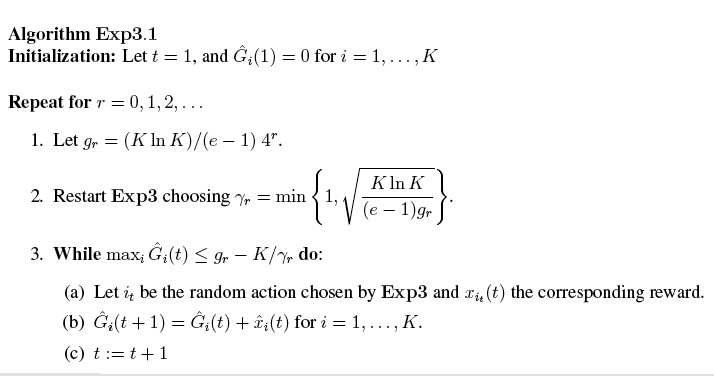
\includegraphics[height=6cm]{figures/Exp3-1.jpg}
\end{frame}

\begin{frame}
\frametitle{Bound for \B{Exp3.1}}
\R{\begin{eqnarray*}
        \Gbest - \E[G_{\Abound}]
&\leq&
8\sqrt{e-1}\sqrt{ \Gbest K \ln K}
+
8(e-1)K
+
2 K \ln K\\
\pause
&\leq&
10.5\;\sqrt{ \Gbest K \ln K}
+
13.8\;K
+
2 K \ln K
\end{eqnarray*}
}
\end{frame}
\section{the non stationary scenario}

\begin{frame}
\frametitle{Allowing switching actions}
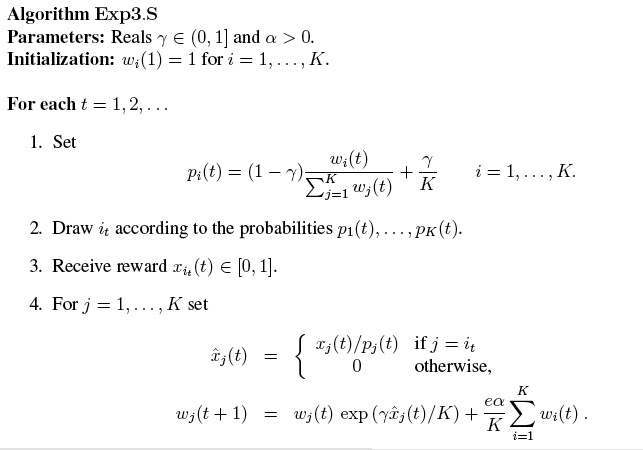
\includegraphics[height=6cm]{figures/Exp3-S.jpg}
\end{frame}

\begin{frame}
\frametitle{Bound for \B{Exp3.S}}
\begin{itemize}
\item \B{Hardness} of sequence $=$ number of switches offline is allowed:
\R{\[
        S \geq \compl(j_1,\ldots,j_T)
        \defeq 1 + \left|\theset{1 \leq \ell < T}{ j_\ell \neq j_{\ell+1}}\right|~.
\]}
\item  Assume \R{$\alpha=1/T$} and
\R{$
        \gamma = \min\braces{1,\sqrt{\frac{K(S\ln(KT)+e)}{(e-1)T}}}~.
$}
\item Then
\R{\[
        G_{j^T} - \E\left[G_{\Aests}\right]
\leq
        2\sqrt{e-1} \sqrt{KT\left(S\ln(KT)+e\right)}
\]}

\end{itemize}
\end{frame}

\section{Combining strategies}

\begin{frame}
\frametitle{Combining strategies}
\begin{itemize}
\item \R{$K$} possible actions and \R{$N$} prediction \B{strategies} or \B{experts}.

\item \R{$N \gg K$}
\item Expert \R{$i$} predicts with \B{a distribution over actions} \R{$\stratv{i}{t} \in [0,1]^K$}
\item Reward of expert \R{$i$} is \R{$\stratv{i}{t}\cdot\xvt$}
\item Considering experts as actions, we get a bound 
\R{$O(\sqrt{g N \log N})$} on the regret.
\item By acting smarter, we can get a bound \R{$O(\sqrt{g K \log N})$}
\end{itemize}
\end{frame}

\begin{frame}
\frametitle{Allowing switching actions}
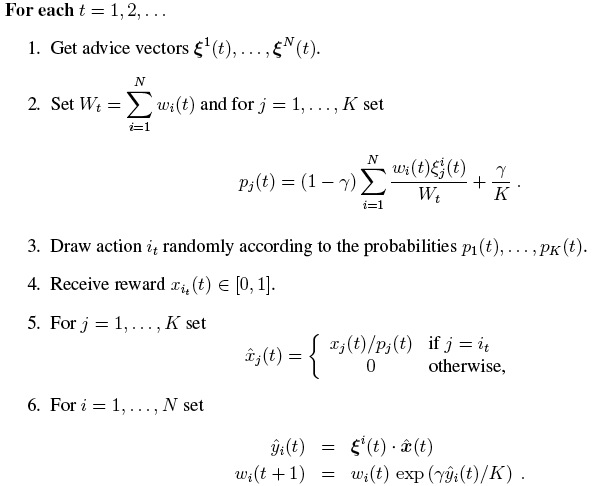
\includegraphics[height=6cm]{figures/Exp4.jpg}
\end{frame}

\section{Summary}

\begin{frame}
\frametitle{Summary}
\begin{itemize}
\item We can achieve diminishing regret even when only gain of chosen action is observable.
\item The increase in the regret is a result of the limited information. 
\R{$ O(\sqrt{TK\log K})$} instead of \R{$ O(\sqrt{T \log K})$}.
\item We can handle non-stationary setups.
\item If we have \B{many} strategies \R{$N$} but only \B{few} actions \R{$K$} we can achieve bounds of the form \R{$O(\sqrt{TK\log N})$}.
\item Example application: choosing a route for an IP packet.
\item \B{Next class}: what happends when both opponents use \hedge?
\end{itemize}
\end{frame}


\iffalse %%%%%%%%%%%%%%%%%%%%%%%%%%%%%%%%%%%%%%%%%%%%%%%%%%%%%%%%%%%%%%%%%%
\begin{frame}
\frametitle{XXX}
\begin{itemize}
\item XXX
\end{itemize}
\end{frame}

\fi %%%%%%%%%%%%%%%%%%%%%%%%%%%%%%%%%%

\end{document}


